

\def\qtr{Winter 2023}
\def\due{Wednesday, January 24 at 11:59 pm}
\def\edstem{\url{https://edstem.org/us/courses/51342/discussion/}}
\def\psetnum{1}

%%% Change the following flag to toggle between questions or solutions
\ifdefined\solutions {} \else \def\solutions{1} \fi


\documentclass{article}

\usepackage{graphicx}

\newcommand{\di}{{d}}
\newcommand{\nexp}{{n}}
\newcommand{\nf}{{p}}
\newcommand{\vcd}{{\textbf{D}}}

\usepackage{nccmath}
\usepackage{mathtools}
\usepackage{graphicx,caption}
\usepackage{enumitem}
\usepackage{epstopdf,subcaption}
\usepackage{psfrag}
\usepackage{amsmath,amssymb,epsf}
\usepackage{verbatim}
\usepackage{url}
\usepackage[hang,flushmargin]{footmisc} 
\usepackage{hyperref}
\newcommand{\hurl}[1]{\href{#1}{#1}}
\renewcommand{\url}{\nolinkurl}
\AtBeginDocument{
	\label{CorrectFirstPageLabel}
	\def\fpage{\pageref{CorrectFirstPageLabel}}
}
\usepackage{color}
\usepackage{bbm}
\usepackage{listings}
\usepackage{setspace}
\usepackage{float}
\usepackage{natbib}
\definecolor{Code}{rgb}{0,0,0}
\definecolor{Decorators}{rgb}{0.5,0.5,0.5}
\definecolor{Numbers}{rgb}{0.5,0,0}
\definecolor{MatchingBrackets}{rgb}{0.25,0.5,0.5}
\definecolor{Keywords}{rgb}{0,0,1}
\definecolor{self}{rgb}{0,0,0}
\definecolor{Strings}{rgb}{0,0.63,0}
\definecolor{Comments}{rgb}{0,0.63,1}
\definecolor{Backquotes}{rgb}{0,0,0}
\definecolor{Classname}{rgb}{0,0,0}
\definecolor{FunctionName}{rgb}{0,0,0}
\definecolor{Operators}{rgb}{0,0,0}
\definecolor{Background}{rgb}{0.98,0.98,0.98}
\lstdefinelanguage{Python}{
numbers=left,
numberstyle=\footnotesize,
numbersep=1em,
xleftmargin=1em,
framextopmargin=2em,
framexbottommargin=2em,
showspaces=false,
showtabs=false,
showstringspaces=false,
frame=l,
tabsize=4,
% Basic
basicstyle=\ttfamily\footnotesize\setstretch{1},
backgroundcolor=\color{Background},
% Comments
commentstyle=\color{Comments}\slshape,
% Strings
stringstyle=\color{Strings},
morecomment=[s][\color{Strings}]{"""}{"""},
morecomment=[s][\color{Strings}]{'''}{'''},
% keywords
morekeywords={import,from,class,def,for,while,if,is,in,elif,else,not,and,or
,print,break,continue,return,True,False,None,access,as,,del,except,exec
,finally,global,import,lambda,pass,print,raise,try,assert},
keywordstyle={\color{Keywords}\bfseries},
% additional keywords
morekeywords={[2]@invariant},
keywordstyle={[2]\color{Decorators}\slshape},
emph={self},
emphstyle={\color{self}\slshape},
%
}


\pagestyle{empty} \addtolength{\textwidth}{1.0in}
\addtolength{\textheight}{0.5in}
\addtolength{\oddsidemargin}{-0.5in}
\addtolength{\evensidemargin}{-0.5in}
\newcommand{\ruleskip}{\bigskip\hrule\bigskip}
\newcommand{\nodify}[1]{{\sc #1}}
\newcommand{\points}[1]{{\textbf{[#1 points]}}}
\newcommand{\subquestionpoints}[1]{{[#1 points]}}
\newenvironment{answer}{{\bf Answer:} \sf \begingroup\color{red}}{\endgroup}%

\newcommand{\bitem}{\begin{list}{$\bullet$}%
{\setlength{\itemsep}{0pt}\setlength{\topsep}{0pt}%
\setlength{\rightmargin}{0pt}}}
\newcommand{\eitem}{\end{list}}

\setlength{\parindent}{0pt} \setlength{\parskip}{0.5ex}
\setlength{\unitlength}{1cm}

\renewcommand{\Re}{{\mathbb R}}
\newcommand{\R}{\mathbb{R}}
\newcommand{\what}[1]{\widehat{#1}}

\renewcommand{\comment}[1]{}
\newcommand{\mc}[1]{\mathcal{#1}}
\newcommand{\half}{\frac{1}{2}}

\def\KL{D_{KL}}
\def\xsi{x^{(i)}}
\def\ysi{y^{(i)}}
\def\zsi{z^{(i)}}
\def\E{\mathbb{E}}
\def\calN{\mathcal{N}}
\def\calD{\mathcal{D}}

\newcommand{\diag}{\mathop{\rm diag}}
\newcommand{\logisticloss}{\ell_{\textup{logistic}}}
\newcommand{\softmax}{\textup{softmax}}
\usepackage{tikz}
\usepackage{bbding}
\usepackage{pifont}
\usepackage{wasysym}
\usepackage{amssymb,amsthm}
\usepackage{booktabs}
\usepackage{verbatim}

\usepackage{algorithmicx}
\usepackage{algpseudocode}
\usepackage{tikz}
\usetikzlibrary{trees}
\usetikzlibrary{arrows.meta, positioning, calc}


\newtheorem{lemma}{Lemma}

\def\shownotes{0}  %set 1 to show author notes
\ifnum\shownotes=1
\newcommand{\authnote}[2]{$\ll$\textsf{\footnotesize #1 notes: #2}$\gg$}
\else
\newcommand{\authnote}[2]{}
\fi

\newcommand{\tnote}[1]{{\color{blue}\authnote{Tengyu}{#1}}}
\newcommand{\fk}[1]{{\color{purple}{[FK:#1]}}}
\newcommand{\notes}[1]{{\color{blue} Note:} \textit{#1} \newline}

\begin{document}

%\pagestyle{myheadings} \markboth{}{CS229 Problem Set \#\psetnum}

\ifnum\solutions=1{
{\huge\noindent CS 229, \qtr\\
Problem Set \#\psetnum}\\\\
YOUR NAME HERE (\texttt{YOUR SUNET HERE})
} \else {\huge
\noindent CS 229, \qtr\\
Problem Set \#\psetnum
} \fi

\ruleskip

{\bf Due {\due } on Gradescope.}

\medskip

\item \points{20} {\bf Decision Trees and Gini Loss}

When growing a decision tree, we split the input space in a greedy, top-down, recursive manner.  Given a parent region $R_p$, we can choose a split $s_p(j, t)$ which yields two child regions $R_1 = \{X \mid x_j < t, X \in R_p\}$ and $R_2 = \{X \mid x_j \geq t, X\in R_p\}$.  Assuming we have defined a per region loss $L(R)$, at each branch we select the split that minimizes the weighted loss of the children:

\begin{align*}
    \min_{j,t} \frac{\lvert R_1 \rvert L(R_1) + \lvert R_2 \rvert L(R_2)}{\lvert R_1 \rvert + \lvert R_2 \rvert}
\end{align*}

When performing classification, a commonly used loss is the Gini loss, defined for the K-class classification problem as:

\begin{align*}
    G(R_m) = G(\vec{p}_m) = \sum_{k=1}^K p_{mk} (1 - p_{mk})
\end{align*}

Where $\vec{p}_m = \begin{bmatrix}p_{m1} & p_{m2} & \dots & p_{mK}\end{bmatrix}$ and $p_{mk}$ is the proportion of examples of class $k$ that are are present in region $R_m$.  However, we are oftentimes more interested in optimizing the final misclassification loss:

\begin{equation}
    \label{misclassificationloss}
    M(R_m) = M(\vec{p}_m) = 1 - \max_k p_{mk} 
\end{equation}

For the problems below, assume we are dealing with binary classification and that there are no degenerate cases where positive and negative datapoints overlap in the feature space.

\begin{enumerate}
    \item \subquestionpoints{5} Show that for any given split, the weighted Gini loss of the children can not exceed that of the parent. (\textbf{Hint}: first show that the Gini loss is strictly concave. And then use the fact that G is strictly concave meaning:
    \begin{align*}
        \forall p_1 \neq p_2, \forall t \in (0, 1): G(t p_1 + (1 - t) p_2) > t G(p_1) + (1 - t) G(p_2)
    \end{align*}
    
	\ifnum\solutions=1 {
	\begin{answer}
\end{answer}
        } \fi
        
    \item \subquestionpoints{5} A multivariate decision tree is a generalization of univariate decision trees, where more than one attribute can be used in the decision rule for each split. For the same data, learn a multivariate decision tree where each decision rule is a linear classifier that makes decisions based on the sign of $\alpha x_{\text{age}} +\beta x_{\text{income}} -1$. Provide a list of all splits with the classification error reduction at each split, as well as $\alpha$, $\beta$. For $\alpha$ and $\beta$, keep two significant decimals.


    
	\ifnum\solutions=1 {
	\begin{answer}
% Accuracy for college degree dataset: 90.0\% \\
% Accuracy for iris dataset: 93.33\% \\
\begin{figure}[H]
    \centering
    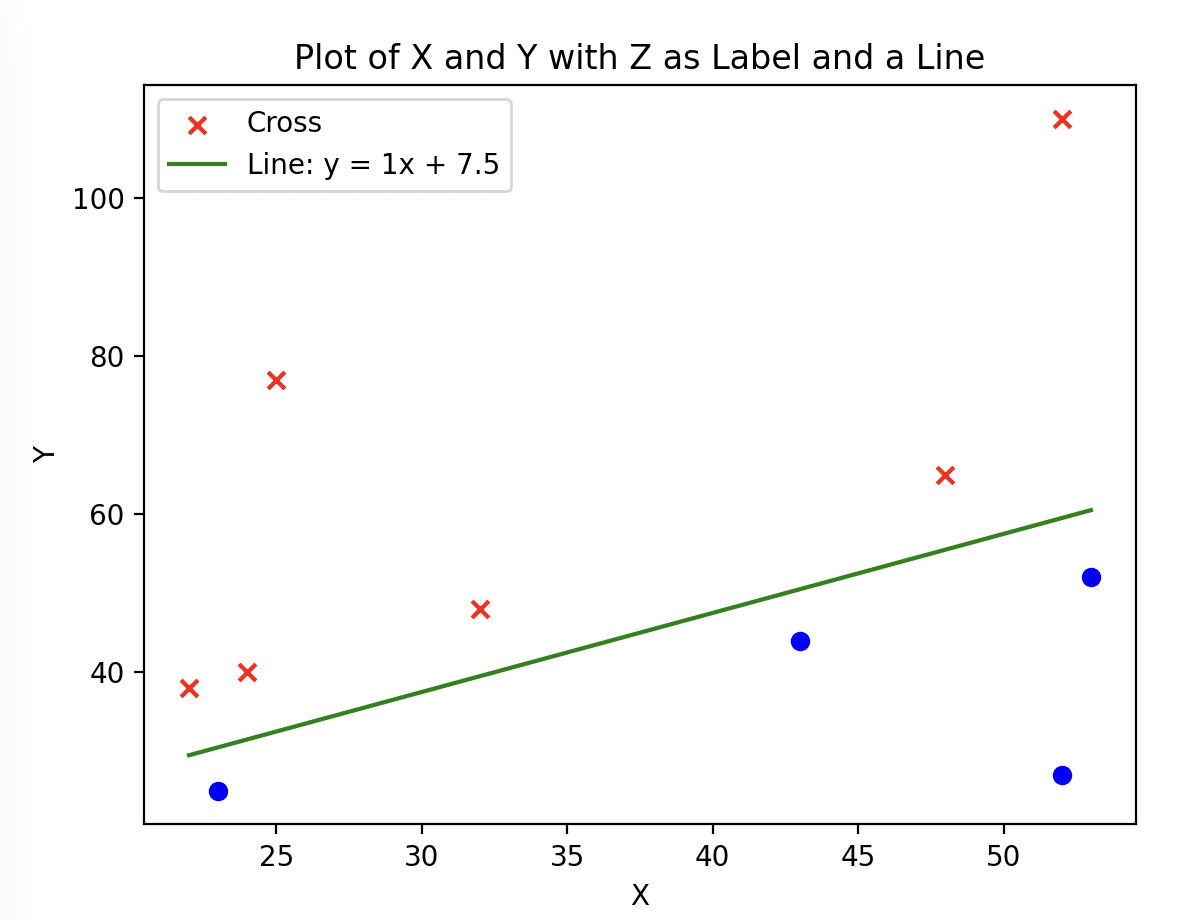
\includegraphics[width=0.5\linewidth]{Screenshot 2024-02-20 at 23.45.57.png}
    \caption{ps3::q1::c}
    \label{fig:enter-label}
\end{figure}

The above figure shows the training samples can be linearly separated by $income = age + 7.5$, this line is equivalent to 
\begin{equation}
    -0.13 \cdot  \text{age} + 0.13 \cdot  \text{income} - 1 = 0
\end{equation}

so $\alpha = -0.13$, $\beta = 0.13$. At root node the classification error is 4, and after one slipt, we get two leaf nodes with classification error = 0
\end{answer}
        } \fi
        
    \item \subquestionpoints{4} If instead we use misclassification loss, what additional case causes the loss to stay the same after a split?  Show why this is (hint: you may find it useful to define $N_m = \lvert R_m \rvert$ and $N_{mk}$ as the number of examples of class $k$ present in $R_m$).
    
	\ifnum\solutions=1 {
	\begin{answer}

Let the parent node $R_p$ have $N_p$ instances in total, with $N_{p1}$ instances of class 1 and $N_{p2}$ instances of class 2, where $N_{p1} > N_{p2}$

The misclassification loss of the parent node is:

\begin{equation}
    M(R_p) = 1 - \frac{N_{p1}}{N_p}
\end{equation}

After the Split, lets assume
\begin{itemize}
    \item \(R_1\) contains \(N_1\) instances, with \(N_{11}\) of class 1 and \(N_{12}\) of class 2.
    \item \(R_2\) contains \(N_2\) instances, with \(N_{21}\) of class 1 and \(N_{22}\) of class 2.
\end{itemize}

The weighted misclassification loss after the split is calculated as:

\begin{equation}
M_{\text{weighted}} = \frac{\lvert R_1 \rvert L(R_1) + \lvert R_2 \rvert L(R_2)}{\lvert R_1 \rvert + \lvert R_2 \rvert} = \frac{N_1 M(R_1) + N_2 M(R_2)}{N_1 + N_2} 
\end{equation}

And 
\begin{equation}
M(R_1) = 1 - \frac{\max(N_{11}, N_{12})}{N_1}
\end{equation}
\begin{equation}
M(R_2) = 1 - \frac{\max(N_{21}, N_{22})}{N_2}
\end{equation}

Replace (9), (10) into (8), and replace $M_{\text{weighted}}$ with (7), we got the the following 
\begin{equation}
\frac{N_1}{N_P}(1 - \frac{\max(N_{11}, N_{12})}{N_1}) + \frac{N_2}{N_P}(1 - \frac{\max(N_{21}, N_{22})}{N_2}) = 1 - \frac{N_{p1}}{N_p}
\end{equation}

Or equivalently, 
\begin{equation}
    N_{p1} = \max(N_{11}, N_{12}) + \max(N_{21}, N_{22})
\end{equation}

so as long as the sum of number of the most frequent classes in two children equals the number of most frequent class in parent, loss will be the same.
\end{answer}
        } \fi
        
    \item \subquestionpoints{6} 
	\vspace{0.2in}
\begin{algorithmic}[1]
    \Function{DecisionTree}{$Data$}
        \If{all points in $Data$ have same label $y$ or max height reached}
            \State \textbf{return} Leaf(majority vote for $y$ in $Data$)
        \Else
            \For{each feature $h_i$}
                \For{each value $v$ of feature $h_i$ in $Data$}
                    \State $Data_1,\ Data_2$ = Split($Data,\ h_i \leq v$)
                    \State $Error_{i, v}$ = ClassificationError($Data_1$) + ClassificationError($Data_2$)
                \EndFor
            \EndFor
            \State $h^*, v^*$ = choose feature $h_i$ and split $v$ that has smallest $Error_{i, v}$
            \State $Data_1,\ Data_2$ = Split($Data,\ h^* \leq v^*$)
            \State \textbf{return} Branch($h^* \leq v^*$, DecisionTree($Data_1$), DecisionTree($Data_2$))
        \EndIf
    \EndFunction
\end{algorithmic}
	
Now imagine we want to predict a person’s salary from their age and whether or not they have a college degree, which is a regression task.  Being the lazy coder you are, you decide to reuse your existing classification tree code above, modifying as few lines as possible to implement a regression tree.
\begin{enumerate}
	\item[(i)] [3 points] Recall that at a leaf node, the decision tree for classification returns the majority vote of training datapoints at that leaf.  For regression, what would an appropriate choice of output be?  Provide the line of code that needs to be modified and write psuedocode for the suggested modification.
	\item[(ii)] [3 points] Recall that the decision tree for classification chooses the split that minimizes classification error. For regression, what would we aim to minimize?  Provide the line of code that needs to be modified and write psuedocode for the suggested modification.
\end{enumerate}
    
	\ifnum\solutions=1 {
	\begin{answer}

(i) 
For regression and predict the salary from college degree and age, we can output the average salary that falls into this node. \\

Changes to make - 1)change the output from a predicted\_class to the average of salary of all its data 2) All reference of node.predicted\_class needs to be corrected to be node.aver\_salary \\
pseudo code as follows\\
    \hspace{10mm} (commented out) predicted\_class = np.argmax(num\_samples\_per\_class) \\
    \hspace{10mm} (commented out) root\_node = Node(predicted\_class=predicted\_class) \\
    root\_node = Node(np.mean(data[index\_of\_salary]))

(ii) 
We still derive a threshold for each split, and minimize the sum of absolute difference between each data and the average of all data in the node. For example, data 1 3 2 fall in the same node, the cost is abs(1 - 2) +  abs(3 - 2) + abs(2 - 2) \\
Changes to make - modify \_misclassification\_loss method \\ 
pseudo code \\
    cost = 0 \\
    aver = mean(data) \\
    for d in data:  cost += abs(data - aver) \\
    return cost
\end{answer}
        } \fi
        
\end{enumerate}


\begin{enumerate}[wide, labelwidth=0pt, labelindent=0pt]

\clearpage
\item \points{20} {\bf Decision Trees and Gini Loss}

When growing a decision tree, we split the input space in a greedy, top-down, recursive manner.  Given a parent region $R_p$, we can choose a split $s_p(j, t)$ which yields two child regions $R_1 = \{X \mid x_j < t, X \in R_p\}$ and $R_2 = \{X \mid x_j \geq t, X\in R_p\}$.  Assuming we have defined a per region loss $L(R)$, at each branch we select the split that minimizes the weighted loss of the children:

\begin{align*}
    \min_{j,t} \frac{\lvert R_1 \rvert L(R_1) + \lvert R_2 \rvert L(R_2)}{\lvert R_1 \rvert + \lvert R_2 \rvert}
\end{align*}

When performing classification, a commonly used loss is the Gini loss, defined for the K-class classification problem as:

\begin{align*}
    G(R_m) = G(\vec{p}_m) = \sum_{k=1}^K p_{mk} (1 - p_{mk})
\end{align*}

Where $\vec{p}_m = \begin{bmatrix}p_{m1} & p_{m2} & \dots & p_{mK}\end{bmatrix}$ and $p_{mk}$ is the proportion of examples of class $k$ that are are present in region $R_m$.  However, we are oftentimes more interested in optimizing the final misclassification loss:

\begin{equation}
    \label{misclassificationloss}
    M(R_m) = M(\vec{p}_m) = 1 - \max_k p_{mk} 
\end{equation}

For the problems below, assume we are dealing with binary classification and that there are no degenerate cases where positive and negative datapoints overlap in the feature space.

\begin{enumerate}
    \item \subquestionpoints{5} Show that for any given split, the weighted Gini loss of the children can not exceed that of the parent. (\textbf{Hint}: first show that the Gini loss is strictly concave. And then use the fact that G is strictly concave meaning:
    \begin{align*}
        \forall p_1 \neq p_2, \forall t \in (0, 1): G(t p_1 + (1 - t) p_2) > t G(p_1) + (1 - t) G(p_2)
    \end{align*}
    
	\ifnum\solutions=1 {
	\begin{answer}
\end{answer}
        } \fi
        
    \item \subquestionpoints{5} A multivariate decision tree is a generalization of univariate decision trees, where more than one attribute can be used in the decision rule for each split. For the same data, learn a multivariate decision tree where each decision rule is a linear classifier that makes decisions based on the sign of $\alpha x_{\text{age}} +\beta x_{\text{income}} -1$. Provide a list of all splits with the classification error reduction at each split, as well as $\alpha$, $\beta$. For $\alpha$ and $\beta$, keep two significant decimals.


    
	\ifnum\solutions=1 {
	\begin{answer}
% Accuracy for college degree dataset: 90.0\% \\
% Accuracy for iris dataset: 93.33\% \\
\begin{figure}[H]
    \centering
    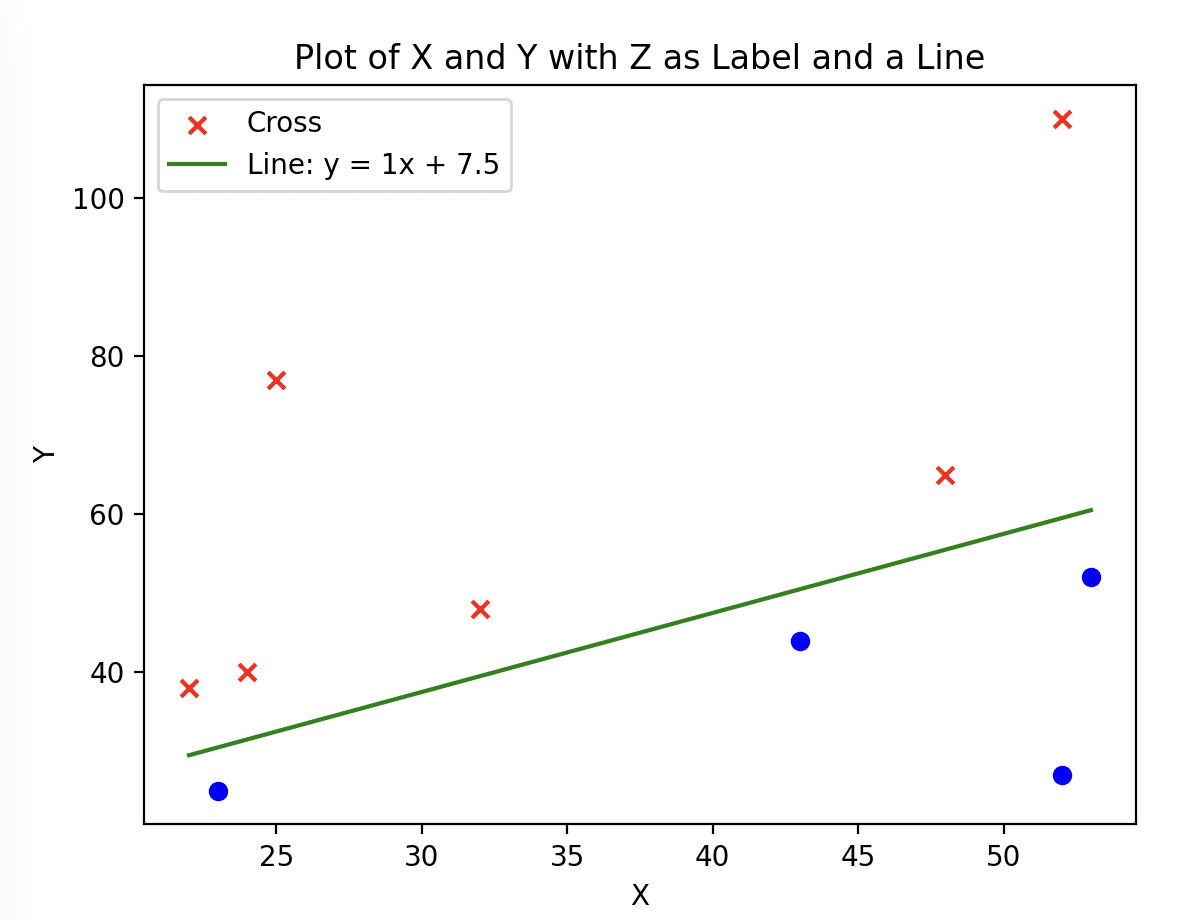
\includegraphics[width=0.5\linewidth]{Screenshot 2024-02-20 at 23.45.57.png}
    \caption{ps3::q1::c}
    \label{fig:enter-label}
\end{figure}

The above figure shows the training samples can be linearly separated by $income = age + 7.5$, this line is equivalent to 
\begin{equation}
    -0.13 \cdot  \text{age} + 0.13 \cdot  \text{income} - 1 = 0
\end{equation}

so $\alpha = -0.13$, $\beta = 0.13$. At root node the classification error is 4, and after one slipt, we get two leaf nodes with classification error = 0
\end{answer}
        } \fi
        
    \item \subquestionpoints{4} If instead we use misclassification loss, what additional case causes the loss to stay the same after a split?  Show why this is (hint: you may find it useful to define $N_m = \lvert R_m \rvert$ and $N_{mk}$ as the number of examples of class $k$ present in $R_m$).
    
	\ifnum\solutions=1 {
	\begin{answer}

Let the parent node $R_p$ have $N_p$ instances in total, with $N_{p1}$ instances of class 1 and $N_{p2}$ instances of class 2, where $N_{p1} > N_{p2}$

The misclassification loss of the parent node is:

\begin{equation}
    M(R_p) = 1 - \frac{N_{p1}}{N_p}
\end{equation}

After the Split, lets assume
\begin{itemize}
    \item \(R_1\) contains \(N_1\) instances, with \(N_{11}\) of class 1 and \(N_{12}\) of class 2.
    \item \(R_2\) contains \(N_2\) instances, with \(N_{21}\) of class 1 and \(N_{22}\) of class 2.
\end{itemize}

The weighted misclassification loss after the split is calculated as:

\begin{equation}
M_{\text{weighted}} = \frac{\lvert R_1 \rvert L(R_1) + \lvert R_2 \rvert L(R_2)}{\lvert R_1 \rvert + \lvert R_2 \rvert} = \frac{N_1 M(R_1) + N_2 M(R_2)}{N_1 + N_2} 
\end{equation}

And 
\begin{equation}
M(R_1) = 1 - \frac{\max(N_{11}, N_{12})}{N_1}
\end{equation}
\begin{equation}
M(R_2) = 1 - \frac{\max(N_{21}, N_{22})}{N_2}
\end{equation}

Replace (9), (10) into (8), and replace $M_{\text{weighted}}$ with (7), we got the the following 
\begin{equation}
\frac{N_1}{N_P}(1 - \frac{\max(N_{11}, N_{12})}{N_1}) + \frac{N_2}{N_P}(1 - \frac{\max(N_{21}, N_{22})}{N_2}) = 1 - \frac{N_{p1}}{N_p}
\end{equation}

Or equivalently, 
\begin{equation}
    N_{p1} = \max(N_{11}, N_{12}) + \max(N_{21}, N_{22})
\end{equation}

so as long as the sum of number of the most frequent classes in two children equals the number of most frequent class in parent, loss will be the same.
\end{answer}
        } \fi
        
    \item \subquestionpoints{6} 
	\vspace{0.2in}
\begin{algorithmic}[1]
    \Function{DecisionTree}{$Data$}
        \If{all points in $Data$ have same label $y$ or max height reached}
            \State \textbf{return} Leaf(majority vote for $y$ in $Data$)
        \Else
            \For{each feature $h_i$}
                \For{each value $v$ of feature $h_i$ in $Data$}
                    \State $Data_1,\ Data_2$ = Split($Data,\ h_i \leq v$)
                    \State $Error_{i, v}$ = ClassificationError($Data_1$) + ClassificationError($Data_2$)
                \EndFor
            \EndFor
            \State $h^*, v^*$ = choose feature $h_i$ and split $v$ that has smallest $Error_{i, v}$
            \State $Data_1,\ Data_2$ = Split($Data,\ h^* \leq v^*$)
            \State \textbf{return} Branch($h^* \leq v^*$, DecisionTree($Data_1$), DecisionTree($Data_2$))
        \EndIf
    \EndFunction
\end{algorithmic}
	
Now imagine we want to predict a person’s salary from their age and whether or not they have a college degree, which is a regression task.  Being the lazy coder you are, you decide to reuse your existing classification tree code above, modifying as few lines as possible to implement a regression tree.
\begin{enumerate}
	\item[(i)] [3 points] Recall that at a leaf node, the decision tree for classification returns the majority vote of training datapoints at that leaf.  For regression, what would an appropriate choice of output be?  Provide the line of code that needs to be modified and write psuedocode for the suggested modification.
	\item[(ii)] [3 points] Recall that the decision tree for classification chooses the split that minimizes classification error. For regression, what would we aim to minimize?  Provide the line of code that needs to be modified and write psuedocode for the suggested modification.
\end{enumerate}
    
	\ifnum\solutions=1 {
	\begin{answer}

(i) 
For regression and predict the salary from college degree and age, we can output the average salary that falls into this node. \\

Changes to make - 1)change the output from a predicted\_class to the average of salary of all its data 2) All reference of node.predicted\_class needs to be corrected to be node.aver\_salary \\
pseudo code as follows\\
    \hspace{10mm} (commented out) predicted\_class = np.argmax(num\_samples\_per\_class) \\
    \hspace{10mm} (commented out) root\_node = Node(predicted\_class=predicted\_class) \\
    root\_node = Node(np.mean(data[index\_of\_salary]))

(ii) 
We still derive a threshold for each split, and minimize the sum of absolute difference between each data and the average of all data in the node. For example, data 1 3 2 fall in the same node, the cost is abs(1 - 2) +  abs(3 - 2) + abs(2 - 2) \\
Changes to make - modify \_misclassification\_loss method \\ 
pseudo code \\
    cost = 0 \\
    aver = mean(data) \\
    for d in data:  cost += abs(data - aver) \\
    return cost
\end{answer}
        } \fi
        
\end{enumerate}


\clearpage
\item \points{20} {\bf Decision Trees and Gini Loss}

When growing a decision tree, we split the input space in a greedy, top-down, recursive manner.  Given a parent region $R_p$, we can choose a split $s_p(j, t)$ which yields two child regions $R_1 = \{X \mid x_j < t, X \in R_p\}$ and $R_2 = \{X \mid x_j \geq t, X\in R_p\}$.  Assuming we have defined a per region loss $L(R)$, at each branch we select the split that minimizes the weighted loss of the children:

\begin{align*}
    \min_{j,t} \frac{\lvert R_1 \rvert L(R_1) + \lvert R_2 \rvert L(R_2)}{\lvert R_1 \rvert + \lvert R_2 \rvert}
\end{align*}

When performing classification, a commonly used loss is the Gini loss, defined for the K-class classification problem as:

\begin{align*}
    G(R_m) = G(\vec{p}_m) = \sum_{k=1}^K p_{mk} (1 - p_{mk})
\end{align*}

Where $\vec{p}_m = \begin{bmatrix}p_{m1} & p_{m2} & \dots & p_{mK}\end{bmatrix}$ and $p_{mk}$ is the proportion of examples of class $k$ that are are present in region $R_m$.  However, we are oftentimes more interested in optimizing the final misclassification loss:

\begin{equation}
    \label{misclassificationloss}
    M(R_m) = M(\vec{p}_m) = 1 - \max_k p_{mk} 
\end{equation}

For the problems below, assume we are dealing with binary classification and that there are no degenerate cases where positive and negative datapoints overlap in the feature space.

\begin{enumerate}
    \item \subquestionpoints{5} Show that for any given split, the weighted Gini loss of the children can not exceed that of the parent. (\textbf{Hint}: first show that the Gini loss is strictly concave. And then use the fact that G is strictly concave meaning:
    \begin{align*}
        \forall p_1 \neq p_2, \forall t \in (0, 1): G(t p_1 + (1 - t) p_2) > t G(p_1) + (1 - t) G(p_2)
    \end{align*}
    
	\ifnum\solutions=1 {
	\begin{answer}
\end{answer}
        } \fi
        
    \item \subquestionpoints{5} A multivariate decision tree is a generalization of univariate decision trees, where more than one attribute can be used in the decision rule for each split. For the same data, learn a multivariate decision tree where each decision rule is a linear classifier that makes decisions based on the sign of $\alpha x_{\text{age}} +\beta x_{\text{income}} -1$. Provide a list of all splits with the classification error reduction at each split, as well as $\alpha$, $\beta$. For $\alpha$ and $\beta$, keep two significant decimals.


    
	\ifnum\solutions=1 {
	\begin{answer}
% Accuracy for college degree dataset: 90.0\% \\
% Accuracy for iris dataset: 93.33\% \\
\begin{figure}[H]
    \centering
    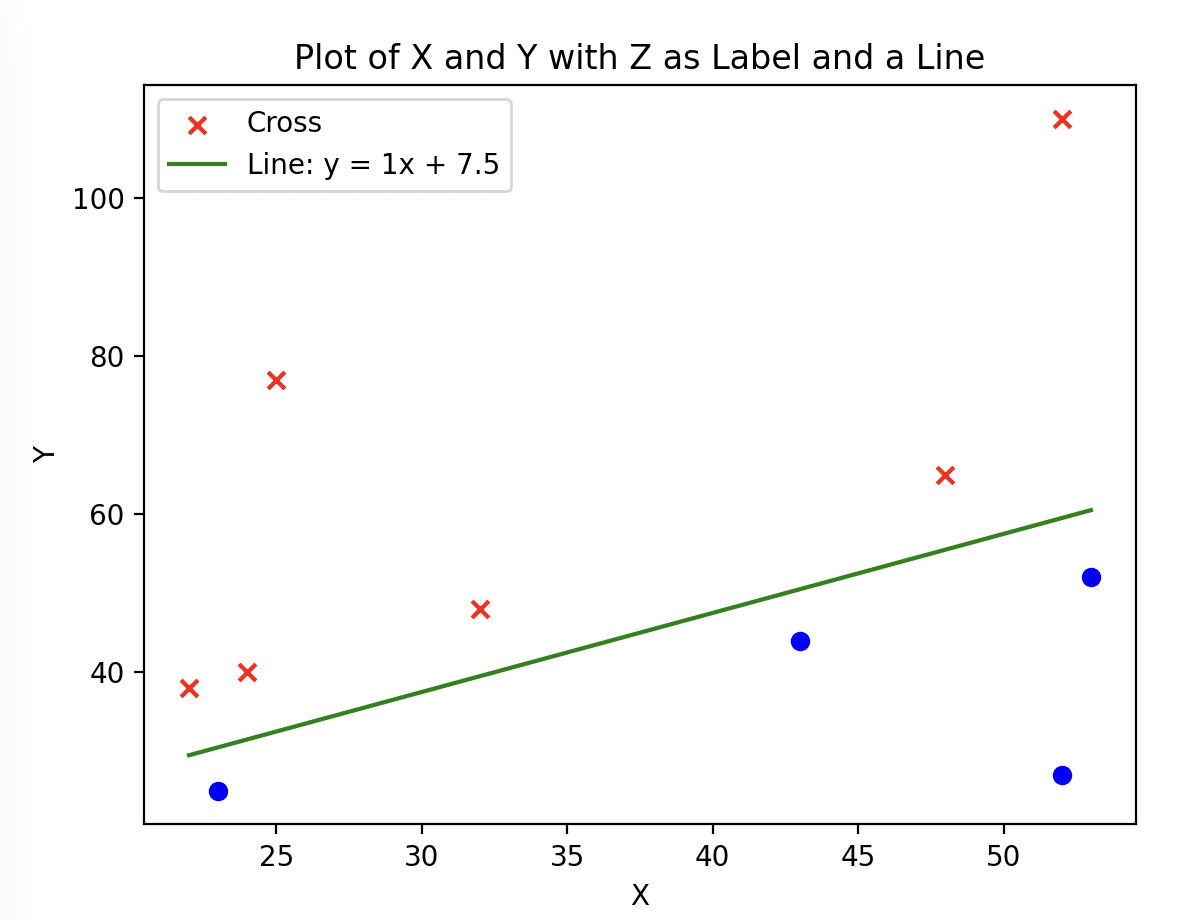
\includegraphics[width=0.5\linewidth]{Screenshot 2024-02-20 at 23.45.57.png}
    \caption{ps3::q1::c}
    \label{fig:enter-label}
\end{figure}

The above figure shows the training samples can be linearly separated by $income = age + 7.5$, this line is equivalent to 
\begin{equation}
    -0.13 \cdot  \text{age} + 0.13 \cdot  \text{income} - 1 = 0
\end{equation}

so $\alpha = -0.13$, $\beta = 0.13$. At root node the classification error is 4, and after one slipt, we get two leaf nodes with classification error = 0
\end{answer}
        } \fi
        
    \item \subquestionpoints{4} If instead we use misclassification loss, what additional case causes the loss to stay the same after a split?  Show why this is (hint: you may find it useful to define $N_m = \lvert R_m \rvert$ and $N_{mk}$ as the number of examples of class $k$ present in $R_m$).
    
	\ifnum\solutions=1 {
	\begin{answer}

Let the parent node $R_p$ have $N_p$ instances in total, with $N_{p1}$ instances of class 1 and $N_{p2}$ instances of class 2, where $N_{p1} > N_{p2}$

The misclassification loss of the parent node is:

\begin{equation}
    M(R_p) = 1 - \frac{N_{p1}}{N_p}
\end{equation}

After the Split, lets assume
\begin{itemize}
    \item \(R_1\) contains \(N_1\) instances, with \(N_{11}\) of class 1 and \(N_{12}\) of class 2.
    \item \(R_2\) contains \(N_2\) instances, with \(N_{21}\) of class 1 and \(N_{22}\) of class 2.
\end{itemize}

The weighted misclassification loss after the split is calculated as:

\begin{equation}
M_{\text{weighted}} = \frac{\lvert R_1 \rvert L(R_1) + \lvert R_2 \rvert L(R_2)}{\lvert R_1 \rvert + \lvert R_2 \rvert} = \frac{N_1 M(R_1) + N_2 M(R_2)}{N_1 + N_2} 
\end{equation}

And 
\begin{equation}
M(R_1) = 1 - \frac{\max(N_{11}, N_{12})}{N_1}
\end{equation}
\begin{equation}
M(R_2) = 1 - \frac{\max(N_{21}, N_{22})}{N_2}
\end{equation}

Replace (9), (10) into (8), and replace $M_{\text{weighted}}$ with (7), we got the the following 
\begin{equation}
\frac{N_1}{N_P}(1 - \frac{\max(N_{11}, N_{12})}{N_1}) + \frac{N_2}{N_P}(1 - \frac{\max(N_{21}, N_{22})}{N_2}) = 1 - \frac{N_{p1}}{N_p}
\end{equation}

Or equivalently, 
\begin{equation}
    N_{p1} = \max(N_{11}, N_{12}) + \max(N_{21}, N_{22})
\end{equation}

so as long as the sum of number of the most frequent classes in two children equals the number of most frequent class in parent, loss will be the same.
\end{answer}
        } \fi
        
    \item \subquestionpoints{6} 
	\vspace{0.2in}
\begin{algorithmic}[1]
    \Function{DecisionTree}{$Data$}
        \If{all points in $Data$ have same label $y$ or max height reached}
            \State \textbf{return} Leaf(majority vote for $y$ in $Data$)
        \Else
            \For{each feature $h_i$}
                \For{each value $v$ of feature $h_i$ in $Data$}
                    \State $Data_1,\ Data_2$ = Split($Data,\ h_i \leq v$)
                    \State $Error_{i, v}$ = ClassificationError($Data_1$) + ClassificationError($Data_2$)
                \EndFor
            \EndFor
            \State $h^*, v^*$ = choose feature $h_i$ and split $v$ that has smallest $Error_{i, v}$
            \State $Data_1,\ Data_2$ = Split($Data,\ h^* \leq v^*$)
            \State \textbf{return} Branch($h^* \leq v^*$, DecisionTree($Data_1$), DecisionTree($Data_2$))
        \EndIf
    \EndFunction
\end{algorithmic}
	
Now imagine we want to predict a person’s salary from their age and whether or not they have a college degree, which is a regression task.  Being the lazy coder you are, you decide to reuse your existing classification tree code above, modifying as few lines as possible to implement a regression tree.
\begin{enumerate}
	\item[(i)] [3 points] Recall that at a leaf node, the decision tree for classification returns the majority vote of training datapoints at that leaf.  For regression, what would an appropriate choice of output be?  Provide the line of code that needs to be modified and write psuedocode for the suggested modification.
	\item[(ii)] [3 points] Recall that the decision tree for classification chooses the split that minimizes classification error. For regression, what would we aim to minimize?  Provide the line of code that needs to be modified and write psuedocode for the suggested modification.
\end{enumerate}
    
	\ifnum\solutions=1 {
	\begin{answer}

(i) 
For regression and predict the salary from college degree and age, we can output the average salary that falls into this node. \\

Changes to make - 1)change the output from a predicted\_class to the average of salary of all its data 2) All reference of node.predicted\_class needs to be corrected to be node.aver\_salary \\
pseudo code as follows\\
    \hspace{10mm} (commented out) predicted\_class = np.argmax(num\_samples\_per\_class) \\
    \hspace{10mm} (commented out) root\_node = Node(predicted\_class=predicted\_class) \\
    root\_node = Node(np.mean(data[index\_of\_salary]))

(ii) 
We still derive a threshold for each split, and minimize the sum of absolute difference between each data and the average of all data in the node. For example, data 1 3 2 fall in the same node, the cost is abs(1 - 2) +  abs(3 - 2) + abs(2 - 2) \\
Changes to make - modify \_misclassification\_loss method \\ 
pseudo code \\
    cost = 0 \\
    aver = mean(data) \\
    for d in data:  cost += abs(data - aver) \\
    return cost
\end{answer}
        } \fi
        
\end{enumerate}


\clearpage
\item \points{20} {\bf Decision Trees and Gini Loss}

When growing a decision tree, we split the input space in a greedy, top-down, recursive manner.  Given a parent region $R_p$, we can choose a split $s_p(j, t)$ which yields two child regions $R_1 = \{X \mid x_j < t, X \in R_p\}$ and $R_2 = \{X \mid x_j \geq t, X\in R_p\}$.  Assuming we have defined a per region loss $L(R)$, at each branch we select the split that minimizes the weighted loss of the children:

\begin{align*}
    \min_{j,t} \frac{\lvert R_1 \rvert L(R_1) + \lvert R_2 \rvert L(R_2)}{\lvert R_1 \rvert + \lvert R_2 \rvert}
\end{align*}

When performing classification, a commonly used loss is the Gini loss, defined for the K-class classification problem as:

\begin{align*}
    G(R_m) = G(\vec{p}_m) = \sum_{k=1}^K p_{mk} (1 - p_{mk})
\end{align*}

Where $\vec{p}_m = \begin{bmatrix}p_{m1} & p_{m2} & \dots & p_{mK}\end{bmatrix}$ and $p_{mk}$ is the proportion of examples of class $k$ that are are present in region $R_m$.  However, we are oftentimes more interested in optimizing the final misclassification loss:

\begin{equation}
    \label{misclassificationloss}
    M(R_m) = M(\vec{p}_m) = 1 - \max_k p_{mk} 
\end{equation}

For the problems below, assume we are dealing with binary classification and that there are no degenerate cases where positive and negative datapoints overlap in the feature space.

\begin{enumerate}
    \item \subquestionpoints{5} Show that for any given split, the weighted Gini loss of the children can not exceed that of the parent. (\textbf{Hint}: first show that the Gini loss is strictly concave. And then use the fact that G is strictly concave meaning:
    \begin{align*}
        \forall p_1 \neq p_2, \forall t \in (0, 1): G(t p_1 + (1 - t) p_2) > t G(p_1) + (1 - t) G(p_2)
    \end{align*}
    
	\ifnum\solutions=1 {
	\begin{answer}
\end{answer}
        } \fi
        
    \item \subquestionpoints{5} A multivariate decision tree is a generalization of univariate decision trees, where more than one attribute can be used in the decision rule for each split. For the same data, learn a multivariate decision tree where each decision rule is a linear classifier that makes decisions based on the sign of $\alpha x_{\text{age}} +\beta x_{\text{income}} -1$. Provide a list of all splits with the classification error reduction at each split, as well as $\alpha$, $\beta$. For $\alpha$ and $\beta$, keep two significant decimals.


    
	\ifnum\solutions=1 {
	\begin{answer}
% Accuracy for college degree dataset: 90.0\% \\
% Accuracy for iris dataset: 93.33\% \\
\begin{figure}[H]
    \centering
    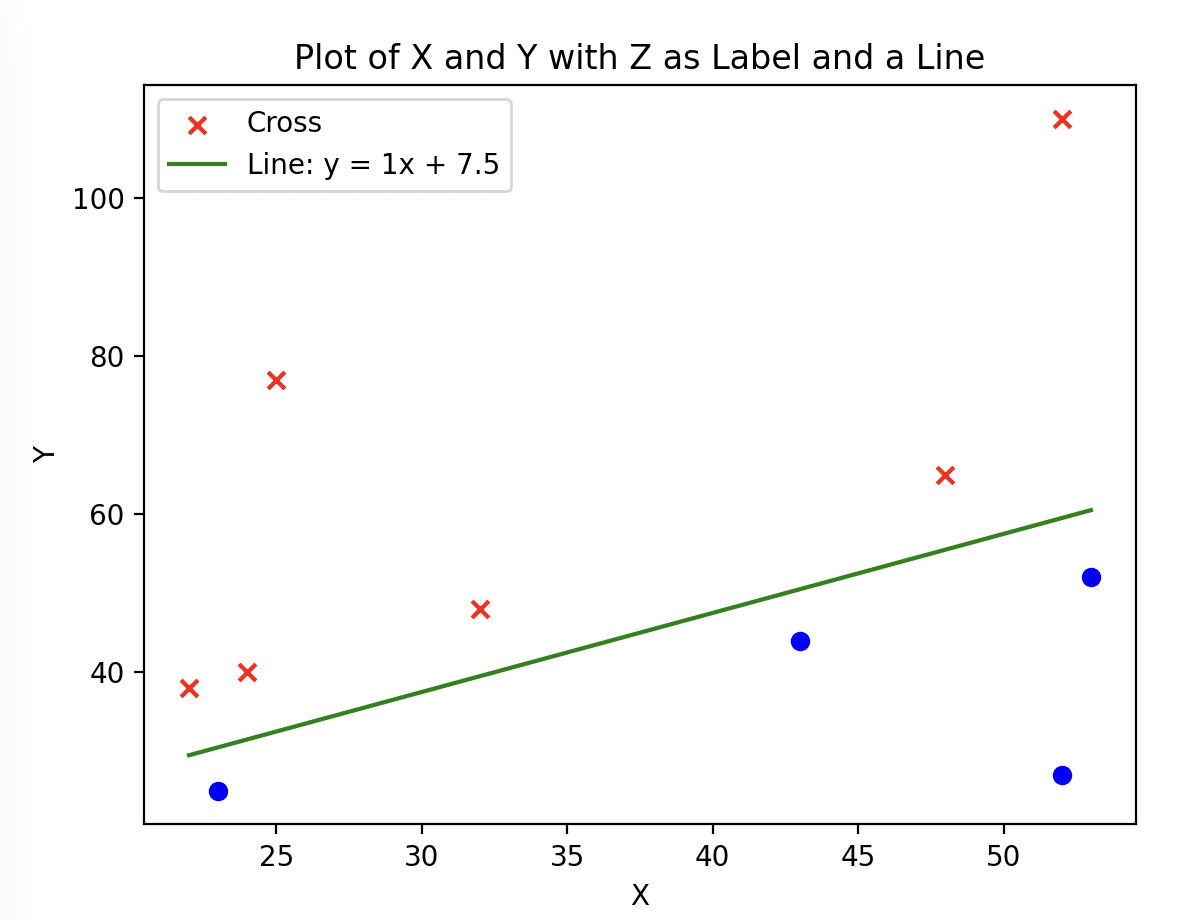
\includegraphics[width=0.5\linewidth]{Screenshot 2024-02-20 at 23.45.57.png}
    \caption{ps3::q1::c}
    \label{fig:enter-label}
\end{figure}

The above figure shows the training samples can be linearly separated by $income = age + 7.5$, this line is equivalent to 
\begin{equation}
    -0.13 \cdot  \text{age} + 0.13 \cdot  \text{income} - 1 = 0
\end{equation}

so $\alpha = -0.13$, $\beta = 0.13$. At root node the classification error is 4, and after one slipt, we get two leaf nodes with classification error = 0
\end{answer}
        } \fi
        
    \item \subquestionpoints{4} If instead we use misclassification loss, what additional case causes the loss to stay the same after a split?  Show why this is (hint: you may find it useful to define $N_m = \lvert R_m \rvert$ and $N_{mk}$ as the number of examples of class $k$ present in $R_m$).
    
	\ifnum\solutions=1 {
	\begin{answer}

Let the parent node $R_p$ have $N_p$ instances in total, with $N_{p1}$ instances of class 1 and $N_{p2}$ instances of class 2, where $N_{p1} > N_{p2}$

The misclassification loss of the parent node is:

\begin{equation}
    M(R_p) = 1 - \frac{N_{p1}}{N_p}
\end{equation}

After the Split, lets assume
\begin{itemize}
    \item \(R_1\) contains \(N_1\) instances, with \(N_{11}\) of class 1 and \(N_{12}\) of class 2.
    \item \(R_2\) contains \(N_2\) instances, with \(N_{21}\) of class 1 and \(N_{22}\) of class 2.
\end{itemize}

The weighted misclassification loss after the split is calculated as:

\begin{equation}
M_{\text{weighted}} = \frac{\lvert R_1 \rvert L(R_1) + \lvert R_2 \rvert L(R_2)}{\lvert R_1 \rvert + \lvert R_2 \rvert} = \frac{N_1 M(R_1) + N_2 M(R_2)}{N_1 + N_2} 
\end{equation}

And 
\begin{equation}
M(R_1) = 1 - \frac{\max(N_{11}, N_{12})}{N_1}
\end{equation}
\begin{equation}
M(R_2) = 1 - \frac{\max(N_{21}, N_{22})}{N_2}
\end{equation}

Replace (9), (10) into (8), and replace $M_{\text{weighted}}$ with (7), we got the the following 
\begin{equation}
\frac{N_1}{N_P}(1 - \frac{\max(N_{11}, N_{12})}{N_1}) + \frac{N_2}{N_P}(1 - \frac{\max(N_{21}, N_{22})}{N_2}) = 1 - \frac{N_{p1}}{N_p}
\end{equation}

Or equivalently, 
\begin{equation}
    N_{p1} = \max(N_{11}, N_{12}) + \max(N_{21}, N_{22})
\end{equation}

so as long as the sum of number of the most frequent classes in two children equals the number of most frequent class in parent, loss will be the same.
\end{answer}
        } \fi
        
    \item \subquestionpoints{6} 
	\vspace{0.2in}
\begin{algorithmic}[1]
    \Function{DecisionTree}{$Data$}
        \If{all points in $Data$ have same label $y$ or max height reached}
            \State \textbf{return} Leaf(majority vote for $y$ in $Data$)
        \Else
            \For{each feature $h_i$}
                \For{each value $v$ of feature $h_i$ in $Data$}
                    \State $Data_1,\ Data_2$ = Split($Data,\ h_i \leq v$)
                    \State $Error_{i, v}$ = ClassificationError($Data_1$) + ClassificationError($Data_2$)
                \EndFor
            \EndFor
            \State $h^*, v^*$ = choose feature $h_i$ and split $v$ that has smallest $Error_{i, v}$
            \State $Data_1,\ Data_2$ = Split($Data,\ h^* \leq v^*$)
            \State \textbf{return} Branch($h^* \leq v^*$, DecisionTree($Data_1$), DecisionTree($Data_2$))
        \EndIf
    \EndFunction
\end{algorithmic}
	
Now imagine we want to predict a person’s salary from their age and whether or not they have a college degree, which is a regression task.  Being the lazy coder you are, you decide to reuse your existing classification tree code above, modifying as few lines as possible to implement a regression tree.
\begin{enumerate}
	\item[(i)] [3 points] Recall that at a leaf node, the decision tree for classification returns the majority vote of training datapoints at that leaf.  For regression, what would an appropriate choice of output be?  Provide the line of code that needs to be modified and write psuedocode for the suggested modification.
	\item[(ii)] [3 points] Recall that the decision tree for classification chooses the split that minimizes classification error. For regression, what would we aim to minimize?  Provide the line of code that needs to be modified and write psuedocode for the suggested modification.
\end{enumerate}
    
	\ifnum\solutions=1 {
	\begin{answer}

(i) 
For regression and predict the salary from college degree and age, we can output the average salary that falls into this node. \\

Changes to make - 1)change the output from a predicted\_class to the average of salary of all its data 2) All reference of node.predicted\_class needs to be corrected to be node.aver\_salary \\
pseudo code as follows\\
    \hspace{10mm} (commented out) predicted\_class = np.argmax(num\_samples\_per\_class) \\
    \hspace{10mm} (commented out) root\_node = Node(predicted\_class=predicted\_class) \\
    root\_node = Node(np.mean(data[index\_of\_salary]))

(ii) 
We still derive a threshold for each split, and minimize the sum of absolute difference between each data and the average of all data in the node. For example, data 1 3 2 fall in the same node, the cost is abs(1 - 2) +  abs(3 - 2) + abs(2 - 2) \\
Changes to make - modify \_misclassification\_loss method \\ 
pseudo code \\
    cost = 0 \\
    aver = mean(data) \\
    for d in data:  cost += abs(data - aver) \\
    return cost
\end{answer}
        } \fi
        
\end{enumerate}


\clearpage
\item \points{20} {\bf Decision Trees and Gini Loss}

When growing a decision tree, we split the input space in a greedy, top-down, recursive manner.  Given a parent region $R_p$, we can choose a split $s_p(j, t)$ which yields two child regions $R_1 = \{X \mid x_j < t, X \in R_p\}$ and $R_2 = \{X \mid x_j \geq t, X\in R_p\}$.  Assuming we have defined a per region loss $L(R)$, at each branch we select the split that minimizes the weighted loss of the children:

\begin{align*}
    \min_{j,t} \frac{\lvert R_1 \rvert L(R_1) + \lvert R_2 \rvert L(R_2)}{\lvert R_1 \rvert + \lvert R_2 \rvert}
\end{align*}

When performing classification, a commonly used loss is the Gini loss, defined for the K-class classification problem as:

\begin{align*}
    G(R_m) = G(\vec{p}_m) = \sum_{k=1}^K p_{mk} (1 - p_{mk})
\end{align*}

Where $\vec{p}_m = \begin{bmatrix}p_{m1} & p_{m2} & \dots & p_{mK}\end{bmatrix}$ and $p_{mk}$ is the proportion of examples of class $k$ that are are present in region $R_m$.  However, we are oftentimes more interested in optimizing the final misclassification loss:

\begin{equation}
    \label{misclassificationloss}
    M(R_m) = M(\vec{p}_m) = 1 - \max_k p_{mk} 
\end{equation}

For the problems below, assume we are dealing with binary classification and that there are no degenerate cases where positive and negative datapoints overlap in the feature space.

\begin{enumerate}
    \item \subquestionpoints{5} Show that for any given split, the weighted Gini loss of the children can not exceed that of the parent. (\textbf{Hint}: first show that the Gini loss is strictly concave. And then use the fact that G is strictly concave meaning:
    \begin{align*}
        \forall p_1 \neq p_2, \forall t \in (0, 1): G(t p_1 + (1 - t) p_2) > t G(p_1) + (1 - t) G(p_2)
    \end{align*}
    
	\ifnum\solutions=1 {
	\begin{answer}
\end{answer}
        } \fi
        
    \item \subquestionpoints{5} A multivariate decision tree is a generalization of univariate decision trees, where more than one attribute can be used in the decision rule for each split. For the same data, learn a multivariate decision tree where each decision rule is a linear classifier that makes decisions based on the sign of $\alpha x_{\text{age}} +\beta x_{\text{income}} -1$. Provide a list of all splits with the classification error reduction at each split, as well as $\alpha$, $\beta$. For $\alpha$ and $\beta$, keep two significant decimals.


    
	\ifnum\solutions=1 {
	\begin{answer}
% Accuracy for college degree dataset: 90.0\% \\
% Accuracy for iris dataset: 93.33\% \\
\begin{figure}[H]
    \centering
    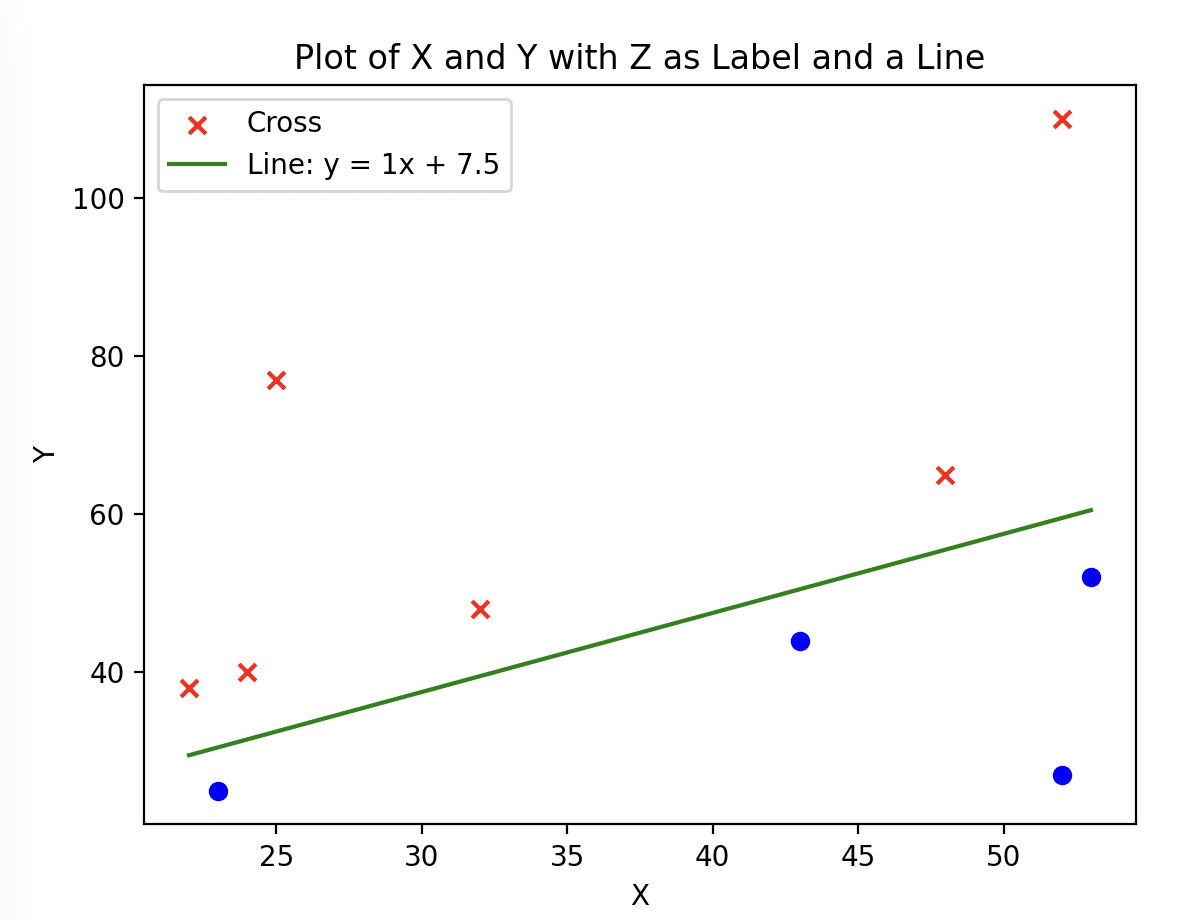
\includegraphics[width=0.5\linewidth]{Screenshot 2024-02-20 at 23.45.57.png}
    \caption{ps3::q1::c}
    \label{fig:enter-label}
\end{figure}

The above figure shows the training samples can be linearly separated by $income = age + 7.5$, this line is equivalent to 
\begin{equation}
    -0.13 \cdot  \text{age} + 0.13 \cdot  \text{income} - 1 = 0
\end{equation}

so $\alpha = -0.13$, $\beta = 0.13$. At root node the classification error is 4, and after one slipt, we get two leaf nodes with classification error = 0
\end{answer}
        } \fi
        
    \item \subquestionpoints{4} If instead we use misclassification loss, what additional case causes the loss to stay the same after a split?  Show why this is (hint: you may find it useful to define $N_m = \lvert R_m \rvert$ and $N_{mk}$ as the number of examples of class $k$ present in $R_m$).
    
	\ifnum\solutions=1 {
	\begin{answer}

Let the parent node $R_p$ have $N_p$ instances in total, with $N_{p1}$ instances of class 1 and $N_{p2}$ instances of class 2, where $N_{p1} > N_{p2}$

The misclassification loss of the parent node is:

\begin{equation}
    M(R_p) = 1 - \frac{N_{p1}}{N_p}
\end{equation}

After the Split, lets assume
\begin{itemize}
    \item \(R_1\) contains \(N_1\) instances, with \(N_{11}\) of class 1 and \(N_{12}\) of class 2.
    \item \(R_2\) contains \(N_2\) instances, with \(N_{21}\) of class 1 and \(N_{22}\) of class 2.
\end{itemize}

The weighted misclassification loss after the split is calculated as:

\begin{equation}
M_{\text{weighted}} = \frac{\lvert R_1 \rvert L(R_1) + \lvert R_2 \rvert L(R_2)}{\lvert R_1 \rvert + \lvert R_2 \rvert} = \frac{N_1 M(R_1) + N_2 M(R_2)}{N_1 + N_2} 
\end{equation}

And 
\begin{equation}
M(R_1) = 1 - \frac{\max(N_{11}, N_{12})}{N_1}
\end{equation}
\begin{equation}
M(R_2) = 1 - \frac{\max(N_{21}, N_{22})}{N_2}
\end{equation}

Replace (9), (10) into (8), and replace $M_{\text{weighted}}$ with (7), we got the the following 
\begin{equation}
\frac{N_1}{N_P}(1 - \frac{\max(N_{11}, N_{12})}{N_1}) + \frac{N_2}{N_P}(1 - \frac{\max(N_{21}, N_{22})}{N_2}) = 1 - \frac{N_{p1}}{N_p}
\end{equation}

Or equivalently, 
\begin{equation}
    N_{p1} = \max(N_{11}, N_{12}) + \max(N_{21}, N_{22})
\end{equation}

so as long as the sum of number of the most frequent classes in two children equals the number of most frequent class in parent, loss will be the same.
\end{answer}
        } \fi
        
    \item \subquestionpoints{6} 
	\vspace{0.2in}
\begin{algorithmic}[1]
    \Function{DecisionTree}{$Data$}
        \If{all points in $Data$ have same label $y$ or max height reached}
            \State \textbf{return} Leaf(majority vote for $y$ in $Data$)
        \Else
            \For{each feature $h_i$}
                \For{each value $v$ of feature $h_i$ in $Data$}
                    \State $Data_1,\ Data_2$ = Split($Data,\ h_i \leq v$)
                    \State $Error_{i, v}$ = ClassificationError($Data_1$) + ClassificationError($Data_2$)
                \EndFor
            \EndFor
            \State $h^*, v^*$ = choose feature $h_i$ and split $v$ that has smallest $Error_{i, v}$
            \State $Data_1,\ Data_2$ = Split($Data,\ h^* \leq v^*$)
            \State \textbf{return} Branch($h^* \leq v^*$, DecisionTree($Data_1$), DecisionTree($Data_2$))
        \EndIf
    \EndFunction
\end{algorithmic}
	
Now imagine we want to predict a person’s salary from their age and whether or not they have a college degree, which is a regression task.  Being the lazy coder you are, you decide to reuse your existing classification tree code above, modifying as few lines as possible to implement a regression tree.
\begin{enumerate}
	\item[(i)] [3 points] Recall that at a leaf node, the decision tree for classification returns the majority vote of training datapoints at that leaf.  For regression, what would an appropriate choice of output be?  Provide the line of code that needs to be modified and write psuedocode for the suggested modification.
	\item[(ii)] [3 points] Recall that the decision tree for classification chooses the split that minimizes classification error. For regression, what would we aim to minimize?  Provide the line of code that needs to be modified and write psuedocode for the suggested modification.
\end{enumerate}
    
	\ifnum\solutions=1 {
	\begin{answer}

(i) 
For regression and predict the salary from college degree and age, we can output the average salary that falls into this node. \\

Changes to make - 1)change the output from a predicted\_class to the average of salary of all its data 2) All reference of node.predicted\_class needs to be corrected to be node.aver\_salary \\
pseudo code as follows\\
    \hspace{10mm} (commented out) predicted\_class = np.argmax(num\_samples\_per\_class) \\
    \hspace{10mm} (commented out) root\_node = Node(predicted\_class=predicted\_class) \\
    root\_node = Node(np.mean(data[index\_of\_salary]))

(ii) 
We still derive a threshold for each split, and minimize the sum of absolute difference between each data and the average of all data in the node. For example, data 1 3 2 fall in the same node, the cost is abs(1 - 2) +  abs(3 - 2) + abs(2 - 2) \\
Changes to make - modify \_misclassification\_loss method \\ 
pseudo code \\
    cost = 0 \\
    aver = mean(data) \\
    for d in data:  cost += abs(data - aver) \\
    return cost
\end{answer}
        } \fi
        
\end{enumerate}


\clearpage
\item \points{20} {\bf Decision Trees and Gini Loss}

When growing a decision tree, we split the input space in a greedy, top-down, recursive manner.  Given a parent region $R_p$, we can choose a split $s_p(j, t)$ which yields two child regions $R_1 = \{X \mid x_j < t, X \in R_p\}$ and $R_2 = \{X \mid x_j \geq t, X\in R_p\}$.  Assuming we have defined a per region loss $L(R)$, at each branch we select the split that minimizes the weighted loss of the children:

\begin{align*}
    \min_{j,t} \frac{\lvert R_1 \rvert L(R_1) + \lvert R_2 \rvert L(R_2)}{\lvert R_1 \rvert + \lvert R_2 \rvert}
\end{align*}

When performing classification, a commonly used loss is the Gini loss, defined for the K-class classification problem as:

\begin{align*}
    G(R_m) = G(\vec{p}_m) = \sum_{k=1}^K p_{mk} (1 - p_{mk})
\end{align*}

Where $\vec{p}_m = \begin{bmatrix}p_{m1} & p_{m2} & \dots & p_{mK}\end{bmatrix}$ and $p_{mk}$ is the proportion of examples of class $k$ that are are present in region $R_m$.  However, we are oftentimes more interested in optimizing the final misclassification loss:

\begin{equation}
    \label{misclassificationloss}
    M(R_m) = M(\vec{p}_m) = 1 - \max_k p_{mk} 
\end{equation}

For the problems below, assume we are dealing with binary classification and that there are no degenerate cases where positive and negative datapoints overlap in the feature space.

\begin{enumerate}
    \item \subquestionpoints{5} Show that for any given split, the weighted Gini loss of the children can not exceed that of the parent. (\textbf{Hint}: first show that the Gini loss is strictly concave. And then use the fact that G is strictly concave meaning:
    \begin{align*}
        \forall p_1 \neq p_2, \forall t \in (0, 1): G(t p_1 + (1 - t) p_2) > t G(p_1) + (1 - t) G(p_2)
    \end{align*}
    
	\ifnum\solutions=1 {
	\begin{answer}
\end{answer}
        } \fi
        
    \item \subquestionpoints{5} A multivariate decision tree is a generalization of univariate decision trees, where more than one attribute can be used in the decision rule for each split. For the same data, learn a multivariate decision tree where each decision rule is a linear classifier that makes decisions based on the sign of $\alpha x_{\text{age}} +\beta x_{\text{income}} -1$. Provide a list of all splits with the classification error reduction at each split, as well as $\alpha$, $\beta$. For $\alpha$ and $\beta$, keep two significant decimals.


    
	\ifnum\solutions=1 {
	\begin{answer}
% Accuracy for college degree dataset: 90.0\% \\
% Accuracy for iris dataset: 93.33\% \\
\begin{figure}[H]
    \centering
    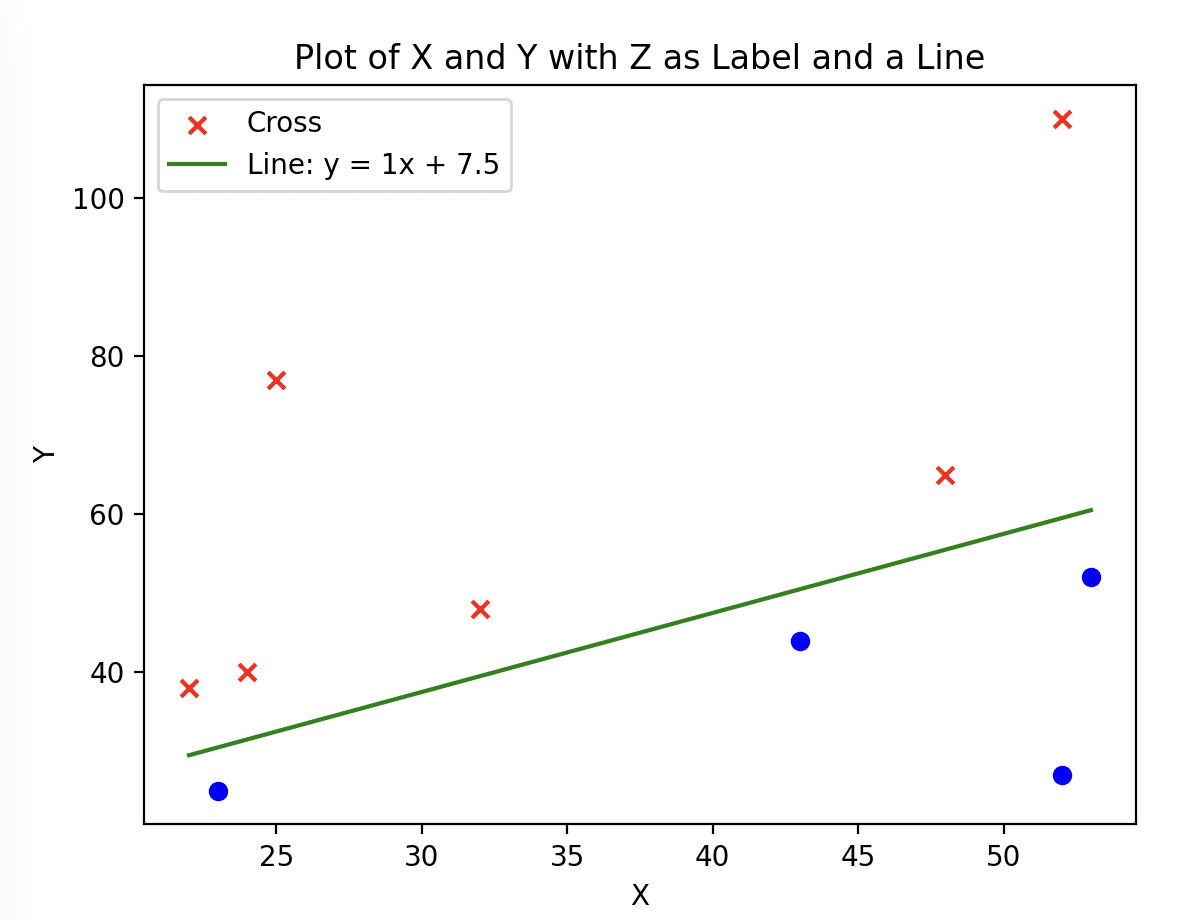
\includegraphics[width=0.5\linewidth]{Screenshot 2024-02-20 at 23.45.57.png}
    \caption{ps3::q1::c}
    \label{fig:enter-label}
\end{figure}

The above figure shows the training samples can be linearly separated by $income = age + 7.5$, this line is equivalent to 
\begin{equation}
    -0.13 \cdot  \text{age} + 0.13 \cdot  \text{income} - 1 = 0
\end{equation}

so $\alpha = -0.13$, $\beta = 0.13$. At root node the classification error is 4, and after one slipt, we get two leaf nodes with classification error = 0
\end{answer}
        } \fi
        
    \item \subquestionpoints{4} If instead we use misclassification loss, what additional case causes the loss to stay the same after a split?  Show why this is (hint: you may find it useful to define $N_m = \lvert R_m \rvert$ and $N_{mk}$ as the number of examples of class $k$ present in $R_m$).
    
	\ifnum\solutions=1 {
	\begin{answer}

Let the parent node $R_p$ have $N_p$ instances in total, with $N_{p1}$ instances of class 1 and $N_{p2}$ instances of class 2, where $N_{p1} > N_{p2}$

The misclassification loss of the parent node is:

\begin{equation}
    M(R_p) = 1 - \frac{N_{p1}}{N_p}
\end{equation}

After the Split, lets assume
\begin{itemize}
    \item \(R_1\) contains \(N_1\) instances, with \(N_{11}\) of class 1 and \(N_{12}\) of class 2.
    \item \(R_2\) contains \(N_2\) instances, with \(N_{21}\) of class 1 and \(N_{22}\) of class 2.
\end{itemize}

The weighted misclassification loss after the split is calculated as:

\begin{equation}
M_{\text{weighted}} = \frac{\lvert R_1 \rvert L(R_1) + \lvert R_2 \rvert L(R_2)}{\lvert R_1 \rvert + \lvert R_2 \rvert} = \frac{N_1 M(R_1) + N_2 M(R_2)}{N_1 + N_2} 
\end{equation}

And 
\begin{equation}
M(R_1) = 1 - \frac{\max(N_{11}, N_{12})}{N_1}
\end{equation}
\begin{equation}
M(R_2) = 1 - \frac{\max(N_{21}, N_{22})}{N_2}
\end{equation}

Replace (9), (10) into (8), and replace $M_{\text{weighted}}$ with (7), we got the the following 
\begin{equation}
\frac{N_1}{N_P}(1 - \frac{\max(N_{11}, N_{12})}{N_1}) + \frac{N_2}{N_P}(1 - \frac{\max(N_{21}, N_{22})}{N_2}) = 1 - \frac{N_{p1}}{N_p}
\end{equation}

Or equivalently, 
\begin{equation}
    N_{p1} = \max(N_{11}, N_{12}) + \max(N_{21}, N_{22})
\end{equation}

so as long as the sum of number of the most frequent classes in two children equals the number of most frequent class in parent, loss will be the same.
\end{answer}
        } \fi
        
    \item \subquestionpoints{6} 
	\vspace{0.2in}
\begin{algorithmic}[1]
    \Function{DecisionTree}{$Data$}
        \If{all points in $Data$ have same label $y$ or max height reached}
            \State \textbf{return} Leaf(majority vote for $y$ in $Data$)
        \Else
            \For{each feature $h_i$}
                \For{each value $v$ of feature $h_i$ in $Data$}
                    \State $Data_1,\ Data_2$ = Split($Data,\ h_i \leq v$)
                    \State $Error_{i, v}$ = ClassificationError($Data_1$) + ClassificationError($Data_2$)
                \EndFor
            \EndFor
            \State $h^*, v^*$ = choose feature $h_i$ and split $v$ that has smallest $Error_{i, v}$
            \State $Data_1,\ Data_2$ = Split($Data,\ h^* \leq v^*$)
            \State \textbf{return} Branch($h^* \leq v^*$, DecisionTree($Data_1$), DecisionTree($Data_2$))
        \EndIf
    \EndFunction
\end{algorithmic}
	
Now imagine we want to predict a person’s salary from their age and whether or not they have a college degree, which is a regression task.  Being the lazy coder you are, you decide to reuse your existing classification tree code above, modifying as few lines as possible to implement a regression tree.
\begin{enumerate}
	\item[(i)] [3 points] Recall that at a leaf node, the decision tree for classification returns the majority vote of training datapoints at that leaf.  For regression, what would an appropriate choice of output be?  Provide the line of code that needs to be modified and write psuedocode for the suggested modification.
	\item[(ii)] [3 points] Recall that the decision tree for classification chooses the split that minimizes classification error. For regression, what would we aim to minimize?  Provide the line of code that needs to be modified and write psuedocode for the suggested modification.
\end{enumerate}
    
	\ifnum\solutions=1 {
	\begin{answer}

(i) 
For regression and predict the salary from college degree and age, we can output the average salary that falls into this node. \\

Changes to make - 1)change the output from a predicted\_class to the average of salary of all its data 2) All reference of node.predicted\_class needs to be corrected to be node.aver\_salary \\
pseudo code as follows\\
    \hspace{10mm} (commented out) predicted\_class = np.argmax(num\_samples\_per\_class) \\
    \hspace{10mm} (commented out) root\_node = Node(predicted\_class=predicted\_class) \\
    root\_node = Node(np.mean(data[index\_of\_salary]))

(ii) 
We still derive a threshold for each split, and minimize the sum of absolute difference between each data and the average of all data in the node. For example, data 1 3 2 fall in the same node, the cost is abs(1 - 2) +  abs(3 - 2) + abs(2 - 2) \\
Changes to make - modify \_misclassification\_loss method \\ 
pseudo code \\
    cost = 0 \\
    aver = mean(data) \\
    for d in data:  cost += abs(data - aver) \\
    return cost
\end{answer}
        } \fi
        
\end{enumerate}


\end{enumerate}

\end{document}
